% +------------------------------------------------------------------------+
% | Reference manual page: Constrained_triangulation_2.tex
% +------------------------------------------------------------------------+
% | 12.04.2000   Author
% | Package: Package
% | 
\RCSdef{\RCSConstrainedtriangulationRev}{$Id$}
\RCSdefDate{\RCSConstrainedtriangulationDate}{$Date$}
% |
%%RefPage: end of header, begin of main body
% +------------------------------------------------------------------------+


\begin{ccRefClass}{Constrained_triangulation_2<Traits,Tds,Itag>}  %% add template arg's if necessary

%% \ccHtmlCrossLink{}     %% add further rules for cross referencing links
%% \ccHtmlIndexC[class]{} %% add further index entries

\ccDefinition  
A constrained triangulation is a triangulation of a set of points
which has to include among its edges 
a given set of segments
joining the points. The given segments are
called {\em constraints}  and the corresponding 
edges in the triangulation are called {\em constrained edges}. 

The endpoints of constrained edges are of course vertices of the
triangulation. However the triangulation may include
include other vertices as well.
There are three versions of  constrained triangulations
\begin{itemize}
\item
In the basic version, the constrained triangulation 
does not handle intersecting constraints, and the set of input 
constraints is required to be a set of segments that do not intersect
except possibly at their endpoints. Any number of constrained edges
are allowed to share the same endpoint.  Vertical constrained edges
are allowed as well as 
constrained edges with null length.
\item
The two other versions support intersecting input constraints.
In those versions, input constraints are allowed to be
intersecting, overlapping or partially
overlapping segments.
The triangulation introduce  additional  vertices at each point which
is a proper intersection point of  two 
constraints. A single constraint intersecting other
constraints will then appear as the union of several 
constrained edges of  the triangulation.
The two versions dealing with intersecting constraints, slightly differ
in the way intersecting constraints are dealt with.
\begin{itemize}
\item  One of them is
designed to be robust when predicates are evaluated exactly but
constructions (i. e.  intersection computations) are
approximate.
\item
The other one is designed to be used 
with an exact arithmetic (meaning exact
evaluation of predicates and exact computation of intersections.)
This last version finds its full efficiency  when used in conjunction
with a constraint hierarchy data structure 
as provided in the class
\ccc{Constrained_triangulation_plus_2}. See
section~\ref{Section_2D_Triangulations_Constrained_Plus}.
\end{itemize}
\end{itemize}



\begin{ccTexOnly}
\begin{center} 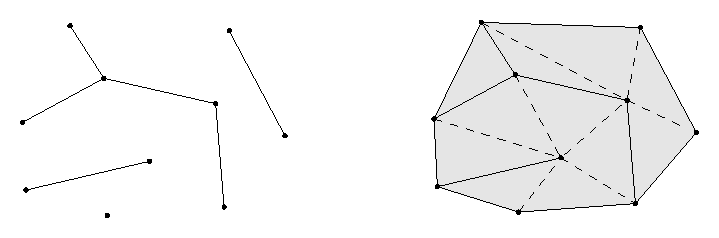
\includegraphics[scale=0.5]{Triangulation_2/constraints} \end{center}
\end{ccTexOnly}

\begin{ccHtmlOnly}
<CENTER>
<img border=0 src="./constraints.gif" align="center" alt="A set of
constraints and its constrained triangulation">
</CENTER>
\end{ccHtmlOnly}

The class \ccRefName\ of the \cgal\ library
implements constrained triangulations.
The template parameter \ccc{Traits} 
stands for a geometric traits class. It has to be a model
of the concept \ccc{TriangulationTraits_2}.
When intersection of input constraints are supported, 
the geometric traits class 
is required to provide additional function object  types
to compute the intersection of two segments.
It has then to be a model of the concept
\ccc{ConstrainedTriangulationTraits_2}.
The template parameter \ccc{Tds}
stands for 
a triangulation data structure class that has to be a model
of the concept \ccc{TriangulationDataStructure_2}.
The third parameter \ccc{Itag} is the intersection tag
which serves  to choose between the different
strategies to deal with constraints intersections. 
\cgal\ provides three valid types for this parameter : \\
\ccc{CGAL::No_intersection_tag} disallows intersections of
 input constraints,\\
\ccc{CGAL::Exact_predicates_tag} is to be used when the traits
class
provides exact predicates but approximate constructions of the
intersection points.\\
\ccc{CGAL::Exact_intersections_tag} is to be used in conjunction
with an exact arithmetic type.

 The information about constrained edges is stored in the 
faces of the triangulation. Thus the nested \ccc{Face}
type of a constrained triangulation offers
additional functionalities to deal with this information.
These additional functionalities 
induce additional requirements on the base face class
plugged into the triangulation data structure of 
 a constrained Delaunay triangulation.
The base face of a constrained Delaunay triangulation
has to be a model of the concept
\ccc{ConstrainedTriangulationFaceBase_2}.

\cgal\ provides  default instantiations for the template parameters
\ccc{Tds} and \ccc{Itag}, and for the \ccc{ConstrainedTriangulationFaceBase_2}.
 If \ccc{Gt} is the geometric traits
parameter,
the default  for
\ccc{ConstrainedTriangulationFaceBase_2}  is the class
\ccc{CGAL::Constrained_triangulation_face_base_2<Gt>}
and the default for the
triangulation data structure parameter is the class
\ccc{CGAL::Triangulation_data_structure_2 <
                       CGAL::Triangulation_vertex_base_2<Gt>,
		       CGAL::Constrained_triangulation_face_base_2<Gt>
>}.
The default intersection tag is \ccc{CGAL::No_intersection_tag}.

\ccInclude{CGAL/Constrained_triangulation_2.h} 
 
\ccInheritsFrom

\ccc{Triangulation_2<Traits,Tds>}

\ccTypes
\ccTypedef{typedef std::pair<Point,Point> Constraint;}{ The type of input
constraints}
\ccTypedef{typedef Itag   Intersection_tag;}{The intersection tag which decides how 
intersections between input constraints are dealt with.}



\ccCreation
\ccCreationVariable{ct}  %% choose variable name

\ccConstructor{Constrained_triangulation_2();}{default constructor.}
\ccConstructor{Constrained_triangulation_2(const
Constrained_triangulation_2& ct1)}
 {Copy constructor, all faces and vertices
are duplicated and  the constrained status of edges
is copied.}


\ccConstructor{ template<class InputIterator> Constrained_triangulation_2(
        InputIterator first,
                               InputIterator last,
                               const Traits& t=Traits());}
{A templated constructor which introduces and builds
 a constrained triangulation with constrained edges in the range 
$\left[\right.$\ccc{first}, \ccc{last}$\left.\right)$.
\ccPrecond The \ccc{value_type} of \ccc{first} and \ccc{last}
 is \ccc{Constraint}.}

\ccHeading{Queries}
\ccMethod{ bool is_constrained(Edge e);}
{Returns true if edge \ccc{e} is a constrained edge.}
\ccMethod{bool are_there_incident_constraints(Vertex_handle v);}
{Returns true if at least one of the edges incident to vertex \ccc{v}
is constrained.}
\ccMethod{template<class OutputItEdges>
  OutputItEdges incident_constraints(Vertex_handle v, 
    OutputItEdges out) const;}
{\ccc{OutputItEdges} is an output iterator with \ccc{Edge} as value
type.
Outputs the constrained edges incident to \ccc{v}
in the sequence pointed to by \ccc{out} and returns the resulting
output iterator.}


\ccHeading{Insertion and removal}

\ccMethod{Vertex_handle insert(Point p, Face_handle f = Face_handle() );}
{ Inserts point \ccc{p} and restores the status (constrained or not) of all
the touched edges. If present \ccc{f} is used as an hint
for the location of \ccc{p}.}

\ccMethod{Vertex_handle 
          insert(const Point& p,
                 Locate_type& lt,
                 Face_handle loc, int li );}
{Same as above except that the location of the point
 \ccc{p} to be inserted is assumed to be given by
\ccc{(lt,loc,i).}}

\ccMethod{Vertex_handle push_back(const Point& p);}
{Equivalent to \ccc{insert(p)}.}

\ccMethod{template < class InputIterator >
          std::ptrdiff_t
          insert(InputIterator first, InputIterator last);}
{Inserts the points in the range
 $\left[\right.$\ccc{first}, \ccc{last}$\left.\right)$.
 Returns the number of inserted points.
 \ccPrecond The \ccc{value_type} of \ccc{first} and \ccc{last}
 is \ccc{Point}.}

\ccMethod{void insert_constraint(Point a, Point b);}
{ Inserts points a and b, and inserts segment ab as a
constraint. Removes the faces crossed by segment ab and creates new
faces instead. If a vertex c lies on segment ab, constraint ab is
replaced by the two constraints ac and \ccc{cb}. Apart from the insertion of
a and b, the algorithm runs in time proportional to the number of
removed triangles. 
\ccPrecond The relative interior of segment \ccc{ab} does not
intersect the relative interior of another constrained edge.}

\ccMethod{ void push_back(const Constraint& c);}
{Inserts constraints \ccc{c} as above.}

\ccMethod{ void insert_constraint(const Vertex_handle & va, const Vertex_handle & vb);}
{ Inserts the line segment \ccc{s} whose endpoints are the vertices 
\ccc{va} and
\ccc{vb}  as a constrained edge \ccc{e}. The triangles intersected by s
are removed and new ones are created.}


\ccMethod{void remove(Vertex_handle v);}
{ Removes a vertex v. 
\ccPrecond Vertex \ccc{v}  is not incident to a constrained edge.}

\ccMethod{ void remove_incident_constraints(Vertex_handle  v);}
{Make the edges incident to vertex \ccc{v} unconstrained edges.}

\ccMethod{void remove_constrained_edge(Face_handle f, int i);}
{ Make edge \ccc{(f,i)}  no longer constrained.}

\begin{ccAdvanced}
\ccMethod{bool
          is_valid(bool verbose = false, int level = 0) const;}
{Checks the validity of the triangulation and
the consistency of the constrained marks in edges.}

\end{ccAdvanced}


\ccHeading{I/O}

\ccFunction{ostream & operator<<(ostream& os, const Constrained_triangulation_2<Traits,Tds> &Ct);}
{Writes the triangulation as for \ccc{CGAL::Triangulation_2<Traits,Tds>} and, for each face f, and integers i=0,1,2,
write ``C'' or ``N'' depending whether edge 
\ccc{(f,i)} is constrained or not.}

\ccFunction{istream& operator>>(istream& is,Constrained_triangulation_2<Traits,Tds> Ct& t);}
{Reads a triangulation from stream \ccc{is} and assigns it to \ccc{t}. Data in the stream must have the same format \ccc{operator<<} uses. 
Note that \ccc{t} is first cleared.}

\ccSeeAlso
\ccc{CGAL::Triangulation_2<Traits,Tds>}, \\
\ccc{TriangulationDataStructure_2}, \\
\ccc{TriangulationTraits_2} \\
\ccc{ConstrainedTriangulationTraits_2} \\
\ccc{ConstrainedTriangulationFaceBase_2} \\




\ccHeading{Implementation}

%The constructors build the triangulation using a sweeping line
%algorithm. The complexity of this algorithm is $O(n\log n)$ if $n$
%endpoints are present. The sweep structure is an \stl\ map.
 The insertion of a constrained edge runs in time
proportional to the number of triangles intersected by this edge.


\end{ccRefClass}

% +------------------------------------------------------------------------+
%%RefPage: end of main body, begin of footer
% EOF
% +------------------------------------------------------------------------+

